\documentclass[11pt]{article}
\usepackage[margin=1in]{geometry}
\usepackage{amsmath,amssymb,amsthm}
\usepackage{mathtools}
\usepackage{graphicx}
\usepackage{booktabs}
\usepackage{multirow}
\usepackage{natbib}
\usepackage{hyperref}
\usepackage{enumitem}
\usepackage{xcolor}
\usepackage[affil-it]{authblk}
\usepackage{setspace}
\usepackage{caption}
\onehalfspacing

\captionsetup[table]{skip=8pt}
\hypersetup{colorlinks=true, linkcolor=blue!50!black, citecolor=blue!50!black, urlcolor=blue!60!black}

\graphicspath{{../figures/}{../code/figures/}}

% Number sections / figures / tables with an "S" prefix so the main
% manuscript can cite them as "Supplementary Figure S1", "Supplementary
% Table S2", etc.
\renewcommand{\thesection}{S\arabic{section}}
\renewcommand{\thefigure}{S\arabic{figure}}
\renewcommand{\thetable}{S\arabic{table}}

\newcommand{\F}{\mathcal{F}}
\newcommand{\N}{N}
\newcommand{\cstar}{c^{\ast}}

\title{\textbf{Supplementary Materials for:\\
Online Traveling Salesman Games: Temporal Nucleolus and the Fragility of the Core under Dynamic Arrivals}}

\author[1]{Seyun Jeong}
\author[2]{Hyunchul Tae}
\affil[1]{Department of Industrial and Management Engineering, Pohang University of Science and Technology (POSTECH), 77 Cheongam-ro, Nam-gu, Pohang, Gyeongbuk 37673, Republic of Korea}
\affil[2]{Korea Institute of Industrial Technology (KITECH), 89 Yangdaegiro-gil, Ipjang-myeon, Seobuk-gu, Cheonan-si, Chungcheongnam-do 31056, Republic of Korea}

\date{\today}

\begin{document}
\maketitle

\section*{Overview}
This document provides supplementary material for the above manuscript. It contains three parts: \S\ref{app:aux} breaks down the aggregate Core-existence rates of the main manuscript's Section~6.4 by arrival pattern and coalition size. \S\ref{app:scale-invariance} documents the empirical verification of the dimensionless joint-rescaling invariance declared in the main manuscript's Section~6.1. \S\ref{app:restricted-lp} details the restricted Core LP methodology used for scale-up instances where $2^n-1$ enumeration is infeasible, together with the full binding-size distributions for the 10 near-complement and 9 intermediate-coalition main-grid cases under nearest-neighbor (NN) dispatch. Theorem, Proposition, Corollary, Remark, and Observation labels below refer to the main manuscript.

\section{Per-pattern Core-existence breakdown}
\label{app:aux}

Figure~\ref{fig:core-n} breaks down the aggregate Core-existence rates of Section~6.4 of the main manuscript by arrival pattern and coalition size $n$. Patterns $\text{B}_{\text{medium}}$, $\text{B}_{\text{light}}$, D, and E retain $100\%$ Core existence across all $n\in\{5,7,10,12,15\}$. Pattern $\text{B}_{\text{heavy}}$ is at $100\%$ for $n\le 10$ and drops to $80\%$ at $n\in\{12,15\}$; the clustered pattern C dips to $80\%$ at $n=10$ and $60\%$ at $n=12$ before recovering to $100\%$ at $n=15$. Simultaneous arrivals (A) collapse from $60\%$ at $n=5$ to $0\%$ at $n=15$. Figure~3 of the main manuscript summarizes this by peak-queue regime $k$.

\begin{figure}[h]
\centering
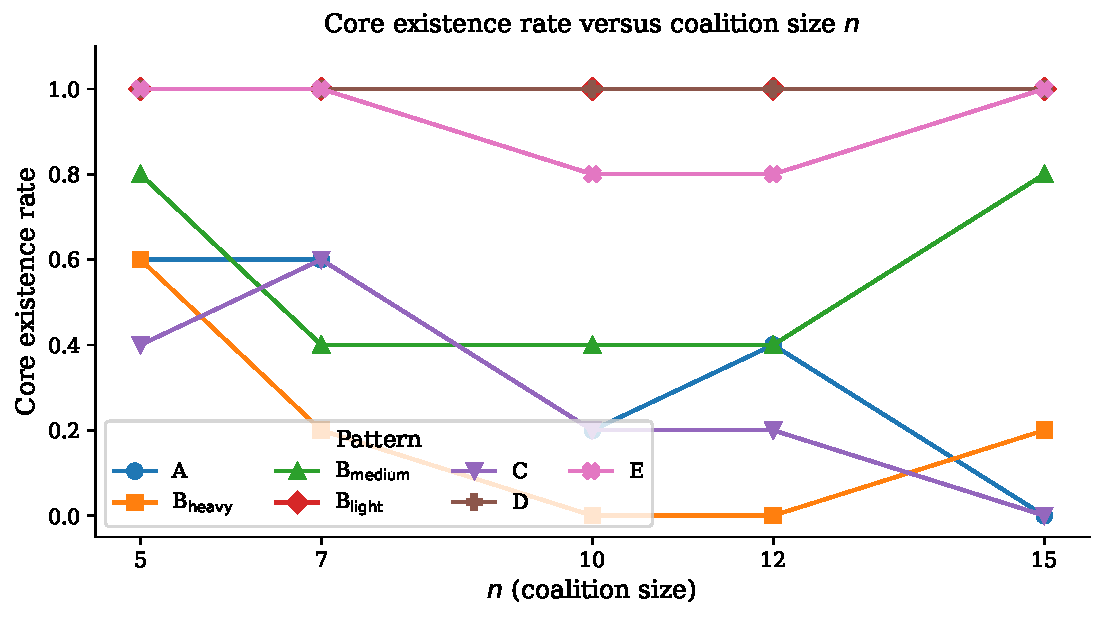
\includegraphics[width=0.75\textwidth]{fig3_core_vs_n.pdf}
\caption{Core-existence rate versus coalition size $n$, broken down by arrival pattern. Patterns $\text{B}_{\text{medium}}$, $\text{B}_{\text{light}}$, D, and E overlap at $1.00$ across the grid. $\text{B}_{\text{heavy}}$ remains at $1.00$ for $n\le 10$ and drops to $0.80$ at $n\in\{12,15\}$; C dips to $0.80$--$0.60$ at $n\in\{10,12\}$ before recovering; simultaneous arrivals (A) collapse to $0\%$ at $n=15$.}
\label{fig:core-n}
\end{figure}

\section{Scale invariance: empirical verification}
\label{app:scale-invariance}

This section verifies empirically the scale invariance stated in Section~6.1 of the main manuscript: that all dimensionless observables are invariant under the joint rescaling $(L, v, \tau) \to (\alpha L, \alpha v, \alpha \tau)$ for any $\alpha > 0$. Since we fix $v = 1$ throughout, this reduces to the simultaneous scaling $(L, \tau) \to (\alpha L, \alpha \tau)$ with the ratio $L/\tau$ (hence the load parameter $\rho$) preserved.

\paragraph{Experimental setup.} Fixing seed $=42$, we generate instances at $n\in\{10,20\}$ and patterns $\{\text{B}_{\text{heavy}},\text{B}_{\text{medium}}, C\}$ under four scale factors $\alpha\in\{0.5,1.0,2.0,5.0\}$. For each configuration, coordinates are sampled from $[0,\alpha\sqrt{n}]^2$ and arrival intervals are scaled from the pattern-prescribed base $\tau_0=\beta_{\mathrm{BHH}}/\rho$ to $\alpha\tau_0$. The nearest-neighbor dispatch policy runs on all 24 instances. Statistics $r$, $r^{\ast\ast}$, and $k$ are recorded.

\paragraph{Results.} Table~\ref{tab:scale-invariance} reports the full 24 instances. For each of the six $(n,\text{pattern})$ configurations, all four $\alpha$ values yield \emph{bit-identical} statistics: the relative standard deviation of $r$ across $\alpha$ is $0$ to machine precision, and $k$ and $r^{\ast\ast}$ are unchanged across $\alpha$ in every configuration. Only the dimensional quantities $L$ and $\tau$ scale linearly with $\alpha$ as expected.

\begin{table}[htbp]
\centering
\footnotesize
\caption{Scale invariance verification (NN policy, seed $=42$). Each row corresponds to one $(n,\text{pattern},\alpha)$ configuration; 24 rows total. Within each $(n,\text{pattern})$ block, the four $\alpha$ values yield identical $r$, $r^{\ast\ast}$, and $k$, confirming joint-rescaling invariance to machine precision. Em-dashes in $r^{\ast\ast}$ indicate configurations where the single-complement threshold of the main manuscript's Theorem~11 is inapplicable (no complement coalition feasible).}
\label{tab:scale-invariance}
\begin{tabular}{@{}cccccccc@{}}
\toprule
$n$ & Pattern & $\alpha$ & $L$ & $\tau$ & $r$ & $r^{\ast\ast}$ & $k$ \\
\midrule
10 & $\text{B}_{\text{heavy}}$ & 0.5 & 1.5811 & 0.0891 & 1.4225 & 1.1324 & 10 \\
10 & $\text{B}_{\text{heavy}}$ & 1.0 & 3.1623 & 0.1781 & 1.4225 & 1.1324 & 10 \\
10 & $\text{B}_{\text{heavy}}$ & 2.0 & 6.3246 & 0.3562 & 1.4225 & 1.1324 & 10 \\
10 & $\text{B}_{\text{heavy}}$ & 5.0 & 15.8114 & 0.8905 & 1.4225 & 1.1324 & 10 \\
\midrule
10 & $\text{B}_{\text{medium}}$ & 0.5 & 1.5811 & 0.1781 & 1.4225 & 1.1324 & 10 \\
10 & $\text{B}_{\text{medium}}$ & 1.0 & 3.1623 & 0.3562 & 1.4225 & 1.1324 & 10 \\
10 & $\text{B}_{\text{medium}}$ & 2.0 & 6.3246 & 0.7124 & 1.4225 & 1.1324 & 10 \\
10 & $\text{B}_{\text{medium}}$ & 5.0 & 15.8114 & 1.7810 & 1.4225 & 1.1324 & 10 \\
\midrule
10 & C & 0.5 & 1.5811 & 0.1781 & 1.2531 & 1.1324 & 10 \\
10 & C & 1.0 & 3.1623 & 0.3562 & 1.2531 & 1.1324 & 10 \\
10 & C & 2.0 & 6.3246 & 0.7124 & 1.2531 & 1.1324 & 10 \\
10 & C & 5.0 & 15.8114 & 1.7810 & 1.2531 & 1.1324 & 10 \\
\midrule
20 & $\text{B}_{\text{heavy}}$ & 0.5 & 2.2361 & 0.0891 & 1.4896 & 1.1039 & 20 \\
20 & $\text{B}_{\text{heavy}}$ & 1.0 & 4.4721 & 0.1781 & 1.4896 & 1.1039 & 20 \\
20 & $\text{B}_{\text{heavy}}$ & 2.0 & 8.9443 & 0.3562 & 1.4896 & 1.1039 & 20 \\
20 & $\text{B}_{\text{heavy}}$ & 5.0 & 22.3607 & 0.8905 & 1.4896 & 1.1039 & 20 \\
\midrule
20 & $\text{B}_{\text{medium}}$ & 0.5 & 2.2361 & 0.1781 & 1.4896 & --- & 17 \\
20 & $\text{B}_{\text{medium}}$ & 1.0 & 4.4721 & 0.3562 & 1.4896 & --- & 17 \\
20 & $\text{B}_{\text{medium}}$ & 2.0 & 8.9443 & 0.7124 & 1.4896 & --- & 17 \\
20 & $\text{B}_{\text{medium}}$ & 5.0 & 22.3607 & 1.7810 & 1.4896 & --- & 17 \\
\midrule
20 & C & 0.5 & 2.2361 & 0.1781 & 1.3469 & 1.1039 & 20 \\
20 & C & 1.0 & 4.4721 & 0.3562 & 1.3469 & 1.1039 & 20 \\
20 & C & 2.0 & 8.9443 & 0.7124 & 1.3469 & 1.1039 & 20 \\
20 & C & 5.0 & 22.3607 & 1.7810 & 1.3469 & 1.1039 & 20 \\
\bottomrule
\end{tabular}
\end{table}

\paragraph{Interpretation.} The absence of variation in $r$, $r^{\ast\ast}$, and $k$ across $\alpha$ confirms that the online arrival process, the NN tour construction, and the Core analysis all depend only on the dimensionless parameters $(n,\rho)$ and are insensitive to the absolute scale of $(L,\tau)$. This justifies the specific choice $L=\sqrt{n}$ adopted in Section~6.1 of the main manuscript without loss of generality.

\section{Restricted Core LP and mechanism classification}
\label{app:restricted-lp}

This section (i) documents the restricted Core LP methodology used for scale-up instances where $2^n-1$ enumeration is infeasible, and (ii) gives the full binding-size distributions for the 10 near-complement and 9 intermediate-coalition main-grid cases under NN.

\paragraph{Motivation (scale-up).} The full Core LP requires one inequality per feasible coalition $S\in\mathcal{F}$, i.e., up to $2^n-1$ constraints. For Pattern~A at $n=30$ this is $\sim 10^9$ and at $n=50$ it is $\sim 10^{15}$, both intractable to enumerate directly.

\paragraph{Sampling strategy.} We solve a \emph{restricted} Core LP over a sampled subset $\mathcal{S}\subseteq\mathcal{F}$: all singletons, all feasible complements $N\setminus\{i\}$, the grand coalition, and $K=10{,}000$ additional random intermediate-size coalitions retained after feasibility filtering. TSP costs $c^{\ast}(S)$ are computed by Held--Karp for $|S|\le 15$ and LKH \citep{helsgaun2000effective} otherwise. The first-stage nucleolus LP
\begin{align}
  \min_{x,\varepsilon}\ \varepsilon\quad\text{s.t.}\quad
  & \sum_i x_i = C(N)_{\text{online}},\qquad
    \sum_{i\in S} x_i - c^{\ast}(S)\le \varepsilon\;\;(S\in\mathcal{S},\ S\ne N) \notag
\end{align}
is solved by CBC via PuLP. If $\varepsilon^{\ast}>0$, $\mathcal{S}$ certifies Core emptiness (the true restricted Core is a subset of the unrestricted Core); the method is one-sided and cannot conclude nonemptiness from a sample.

\paragraph{Scale-up certification (Pattern A seed 123).} After the Phase-4 simulator corrections, the earlier 5-case study collapses to the 2 cases at $n=20, 30$ where seed 123 under Pattern A still eludes the main manuscript's Theorem~11:
\begin{center}
\footnotesize
\begin{tabular}{@{}lccccccc@{}}
\toprule
Pattern & $n$ & Seed & $r$ & $r^{\ast\ast}$ & $\varepsilon^{\ast}$ & Binding sizes & Mechanism \\
\midrule
A & 20 & 123 & 1.077 & 1.112 & $0.77$ & $\{n-2,\,n-1\}$ & near-complement \\
A & 30 & 123 & 1.038 & 1.088 & $0.66$ & $\{n-2,\,n-1\}$ & near-complement \\
\bottomrule
\end{tabular}
\end{center}
The remaining seed-123 scale-up cases at $n=50$ (and at $n\in\{20,30,50\}$ under Pattern~C) now fire the main manuscript's Theorem~11 directly and do not require the restricted-LP certificate.

\paragraph{Main-grid near-complement cases (main manuscript, Remark~14).} Table~\ref{tab:near-main} lists the 10 NN main-grid instances classified as near-complement by the first-stage LP's binding-size distribution.

\begin{table}[htbp]
\centering
\footnotesize
\caption{Ten main-grid NN instances in the near-complement class (main manuscript, Remark~14). The main manuscript's Theorem~11 and Proposition~12 are both vacuous (or the latter inapplicable). Tight binding concentrates at sizes $\{n-2, n-1\}$.}
\label{tab:near-main}
\begin{tabular}{@{}rllrrrrr@{}}
\toprule
$n$ & pattern & seed & $k$ & $r$ & $r^{\ast\ast}$ & $r^{\ast\ast\ast}$ & binding at $n-2, n-1$ \\
\midrule
10 & A        & 123 & 10 & 1.053 & 1.150 & 1.053 & yes \\
10 & B\_heavy & 256 & 10 & 1.126 & 1.138 & 1.061 & yes \\
10 & C        & 123 & 10 & 1.124 & 1.150 & 1.053 & yes \\
15 & A        &  42 & 15 & 1.048 & 1.121 & 1.051 & yes \\
15 & A        &  99 & 15 & 1.051 & 1.151 & 1.043 & yes \\
15 & A        & 123 & 15 & 1.075 & 1.145 & 1.042 & yes \\
15 & B\_heavy &   7 & 15 & 1.185 & 1.194 & 1.046 & yes \\
15 & C        &  42 & 15 & 1.068 & 1.121 & 1.051 & yes \\
15 & C        &  99 & 15 & 1.148 & 1.151 & 1.043 & yes \\
15 & C        & 123 & 15 & 1.141 & 1.145 & 1.042 & yes \\
\bottomrule
\end{tabular}
\end{table}

\paragraph{Main-grid intermediate cases (main manuscript, Observation~15).} Table~\ref{tab:inter-binding} gives the full binding-size distribution for the 9 intermediate instances. Binding concentrates on sizes $|S|\in\{3,\ldots,n-3\}$, with no size-$(n-1)$ or size-$(n-2)$ involvement.

\begin{table}[htbp]
\centering
\footnotesize
\caption{Nine main-grid NN instances in the intermediate-coalition class (main manuscript, Observation~15). The ``binding sizes'' column lists $|S|=c$ pairs, meaning $c$ constraints of size $|S|$ are tight at the first-stage LP optimum.}
\label{tab:inter-binding}
\begin{tabular}{@{}rllrrrl@{}}
\toprule
$n$ & pattern & seed & $k$ & $r$ & $\varepsilon^{\ast}$ & binding sizes (count) \\
\midrule
 7 & B\_medium & 256 &  5 & 1.436 & 0.028 & $\{1{=}1,\,2{=}1,\,3{=}4,\,4{=}6,\,5{=}2\}$ \\
10 & B\_medium & 123 &  8 & 1.423 & 0.192 & $\{1{=}1,\,2{=}3,\,3{=}6,\,4{=}9,\,5{=}9,\,6{=}5,\,7{=}1\}$ \\
10 & B\_medium & 256 &  8 & 1.358 & 0.217 & $\{1{=}2,\,2{=}2,\,3{=}1,\,4{=}2,\,5{=}1,\,6{=}3,\,7{=}3,\,8{=}1\}$ \\
10 & E        &  42 &  8 & 1.495 & 0.062 & $\{1{=}1,\,2{=}1,\,3{=}5,\,4{=}3,\,5{=}3,\,6{=}2,\,7{=}1\}$ \\
12 & B\_medium &  99 & 10 & 1.395 & 0.744 & $\{3{=}2,\,4{=}2,\,5{=}6,\,6{=}12,\,7{=}12,\,8{=}6,\,9{=}1\}$ \\
12 & B\_medium & 123 & 10 & 1.487 & 0.767 & $\{1{=}1,\,2{=}1,\,3{=}2,\,4{=}2,\,5{=}6,\,6{=}9,\,7{=}7,\,8{=}4,\,9{=}1\}$ \\
12 & B\_medium & 256 & 10 & 1.423 & 0.941 & $\{1{=}1,\,2{=}1,\,6{=}3,\,7{=}9,\,8{=}9,\,9{=}5,\,10{=}1\}$ \\
12 & E        &  42 &  9 & 1.610 & 0.289 & $\{3{=}4,\,4{=}5,\,5{=}5,\,6{=}5,\,7{=}3,\,8{=}1\}$ \\
15 & B\_medium & 256 & 12 & 1.326 & 0.185 & $\{1{=}1,\,2{=}1,\,3{=}3,\,4{=}2,\,7{=}1,\,8{=}5,\,9{=}7,\,10{=}7,\,11{=}2,\,12{=}1\}$ \\
\bottomrule
\end{tabular}
\end{table}

\paragraph{Interpretation.} The near-complement table (Table~\ref{tab:near-main}) confirms that the 10 main manuscript's Remark~14 cases share the signature $\{n-2, n-1\}$ binding: neither size alone certifies emptiness, but the combined presence of both sizes does. The intermediate table (Table~\ref{tab:inter-binding}) shows that the 9 Observation~15 cases have binding concentrated on small-to-medium coalition sizes, with $r\in[1.33,1.61]$ and $k<n-1$ in every case. A tight analytic sufficient condition for either class remains open (main manuscript, Section~7).

\bibliographystyle{plainnat}
\bibliography{references}

\end{document}
